\chapter{Resultados}

En este capítulo pasamos a detallar los resultados de todos y cada uno de los análisis realizados.

\section{Análisis general de la plataforma}

La plataforma Prado usa la versión 2.6.4 de \textit{Moodle}, aunque la última versión estable a 15 de mayo de 2017 es la 3.3. La rama 2.6 dejó de recibir actualizaciones de soporte hace 2 años. Para conocer la versión de prado se puede consultar la url \url{http://prado.ugr.es/moodle/lib/upgrade.txt}.

\bigskip
Prado2 usa como plantilla el tema \textit{Archaius} \cite{moodletheme}, desarrollada por el programador colombiano Daniel Múnera Sánchez. Podemos ver la versión de la plantilla accediendo a \url{http://prado.ugr.es/moodle/theme/archaius/README.md} y viendo que la versión instalada es del 11 de agosto de 2014, cuando dicho tema tiene versiones más actualizadas que solucionan diversos problemas.

\bigskip
Nos pusimos en contacto con el desarrollador de la plantilla, y muy amablemente nos contestó a todas las dudas que teníamos sobre la misma. También nos confirmó que había abandonado el desarrollo de la plantilla por falta de tiempo con lo que no habrá más actualizaciones de la misma.

\bigskip
Al acceder a la url \url{http://prado.ugr.es/} nuestro navegador descargará un archivo \texttt{index.html} (ver figura \ref{redireccionhttp}), cuya única función es redireccionar al subdirectorio \texttt{/moodle/}. las redirecciones HTTP están desaconsejadas y hay otras formas más apropiadas de resolver este problema utilizando una única petición HTTP. Por experiencia propia, esto deja entrever que se partió de una instalación rápida desempaquetando el fichero comprimido de \textit{Moodle} y empezando a trabajar desde ahí. A primera vista, parece que se ha hecho así para hacer referencia a que se está usando el paquete \textit{Moodle} pero se han eliminado todas las referencias al mismo, incluso los enlaces a su licencia, cosa a la que obliga la GPLv3, licencia de \textit{Moodle}.

\bigskip
Curiosamente Ágora \url{http://pefc5.ugr.es}, que es la instalación de \textit{Moodle} que utilizan en la facultad de psicología, resuelve esto con una redirección 302.

\bigskip
En cuanto al motor de base de datos, desde el CEVUG nos comentaron que utilizaban \textit{Oracle} por requerimiento del CSIRC, pues no daban soporte a ningún otro motor de base de datos y además habían tenido que realizar diversas adaptaciones al código de \textit{Moodle} para que funcionara sobre este motor. Tras la recepción de los datos por parte del CEVUG y analizando la consulta que lanzaron para obtener los datos, pudimos certificar que efectivamente estaban usando \textit{Oracle}, pues la consulta hacía uso de funciones propias de \textit{Oracle}, pero que \textit{Moodle} soporta de forma nativa 4 motores de base de datos: MySQL, PostgreSqL, MSSQL y Oracle, por lo que suponemos que las adaptaciones serían para automatizar la creación de cursos, alumnos y profesores.  


\begin{figure}
\centering
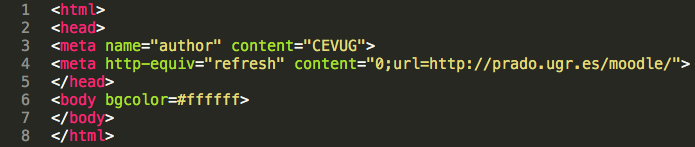
\includegraphics[width=1.0\textwidth]{../screenshots/redireccionhttp}
\caption{Redireccion HTTP al acceder a http://prado.ugr.es}
\label{redireccionhttp}
\end{figure}

\bigskip
Las versiones antiguas de \textit{Moodle} utilizaban la librería YUI, desarrollada por \textit{Yahoo} y cuyo desarrollo se abandonó el 29 de agosto de 2014 \cite{art_01}. A partir de la versión 2.9 se comenzó a migrar a la librería jQuery. Aunque \textit{Moodle} 2.6 utiliza YUI, la plantilla Archaius usa varias funciones de la librería jQuery 1.10.2 \url{https://prado.ugr.es/moodle/theme/jquery.php/core/jquery-1.10.2.min.js} que fue liberada el 3 de Julio de 2013 y que, teniendo en cuenta que la librería está ya por su versión 3.2, vemos que está claramente obsoleta.

\bigskip
Se está utilizando Apache como servidor HTTP, notar que se oculta su versión haciéndolo mas seguro ante posibles ataques dirigidos, esto es un acierto.

\bigskip
El servidor tiene instalada la versión 5.4.45 que fue liberada el 3 de septiembre de 2015 y que, como podemos ver en \url{http://php.net/supported-versions.php}, ya no está soportada. En este caso hay dos problemas, por un lado el usar una versión tan anticuada de PHP y por otra no ocultar la versión, siendo muy fácil encontrar vulnerabilidades para dicha versión.

\section{Entrevistas personales}

Como ya hemos comentado, se hicieron una serie de entrevistas informales. Dichas entrevistas consistían en anotar tanto los puntos de vista de los usuarios como sus quejas y sugerencias. Al finalizar, se hacía un pequeño test de usabilidad consistente en pedir a los usuarios que cambiaran su foto de perfil de \textit{Prado2}. En el test participaron cerca de 30 personas: tanto profesores y usuarios de \textit{Prado2} como gente externa que nunca había visto la plataforma.

\bigskip
Para cambiar la imagen de perfil de \textit{Prado2} la ruta correcta a seguir es:

\begin{center}
Administración $\rightarrow$ Editar Perfil $\rightarrow$ Imagen del Usuario 
\end{center}

y aunque puede parecer sencillo, nadie bajó del minuto y medio mientras probaba erráticamente varias rutas. Hubo un estudiante del Grado en Ingeniería Informática que tardó más de 4 minutos.

\bigskip
Todos los usuarios repetían el mismo patrón: como se les pedía que cambiaran la imagen del perfil, lo primero que hacían era hacer click en la imagen de perfil para ver si salía alguna opción de editar. Esto deja entrever lo lejos que está la plantilla actual del uso real que hacen los usuarios. 

\bigskip
Además los distintos usuarios nos hicieron notar los siguientes problemas y/o carencias con los que se habían encontrado:

\begin{enumerate}

\item Es imposible desmatricularse de asignaturas de otros cursos o de las que el alumno ha cambiado de grupo.

\item Aunque se escoja como idioma el inglés hay muchas cosas que aparecen en castellano, de hecho están mezclados ambos idiomas

\item La ventana de solicitud de contraseña de \textit{Prado2} (el IDP del CSIRC) coge la configuración de idioma del navegador del usuario en lugar de la que viene de Prado. Esto hace que si por ejemplo tu navegador está en inglés pero tu estás mostrando Prado en español, al acceder al IDP la ventana se muestre en inglés.

\item Hay que descargar los materiales de la asignatura uno a uno en lugar de dar una opción para descargar todo el conjunto en un archivo comprimido.

\item Si se está navegando por la miga de pan se llegan a mostrar unos listados de asignaturas con mas de mil registro haciendo inusable el seleccionar alguna

\item El menú superior de asignaturas es inusable por los profesores pues no saben a ciencia cierta a qué asignatura están accediendo hasta que han hecho click, ya que muchas asignaturas comparten nombre simplemente cambiando los profesores.

\item No se notifican los cambios y/o novedades en la plataforma. Esto hace que a veces se cambie algo que funcionaba de una determinada manera y provoque confusión.

\item Si un alumno contiene un carácter no ASCII, como pueden ser vocales acentuadas o una ``ñ'', a la hora de descargar los trabajos de dicho alumno la codificación del archivo será incorrecta y al desempaquetar el archivo .zip en sistemas windows aparece una carpeta vacía (en sistemas Linux no hay problema). En este caso el profesor recibió una queja del alumno por que no le habían calificado una serie de ejercicios. El profesor estuvo haciendo comprobaciones en varios sistemas y lo puso en conocimiento del CSIRC, donde le aseguraron que era problema de su equipo. 

\item En determinados listados, no aparecen barras de desplazamiento horizontal por lo que aparece la información cortada. En otros listados, al contrario, dichas barras son tan largas que en numerosas ocasiones se ha perdido la localización espacial de la fila y se ha puntuado al alumno incorrecto.

\item Hay diferentes vistas de la ventana ``Mis cursos'' con la consecuente confusión

\item No se notifica a los usuarios cuando hay material nuevo o modificado, obligando a comprobar periódicamente el material uno a uno.

\item Las calificaciones finales no se muestran aunque el profesor las publique.

\item A la hora de mostrar las calificaciones, salen trozos de pruebas ocultas de otros cursos y otros grupos sin rellenar.

\item No se notifican la convocatorias de exámenes.

\item El sistema de mensajería es complicado de encontrar y mucho más complicado de usar. En primer lugar, el profesor ha de marcar uno a uno los alumnos no habiendo una opción para seleccionarlos todos. Además, en lugar de aparecer un botón que ponga  ``Enviar mensaje'', aparece un desplegable cuya única opción es ``Enviar mensaje'' (ver imagen \ref{fig:pantallazoPradoenviarMensaje}), al seleccionar esa opción pasamos a una ventana donde podemos redactar el mensaje, aunque las opciones de insertar elementos no funcionan correctamente. En la parte inferior de ese mensaje vemos que aparece de nuevo toda la lista de alumnos sin respetar los que se habían marcado previamente. Al enviar el mensaje, el profesor no recibe una copia pese a haberse marcado, con lo que no puede comprobar que efectivamente se está enviado el mensaje a todos los alumnos. El editor de mensajes no deja copiar/pegar con el botón derecho del ratón aunque si que deja hacerlo mediante atajos de teclado. Por último, y no menos importante, no permite editar el asunto del mensaje. Si además sucede algún problema al enviar mensajes a los alumnos, nos podemos encontrar con un críptico mensaje de error como el de la figura \ref{fig:pantallazoPradoMensaje2} que dice  ``Algo ha ido mal al enviar mensajes a los usuarios seleccionados. Algunos pueden haber recibido el mensaje''.


\begin{figure}[h!]
\centering
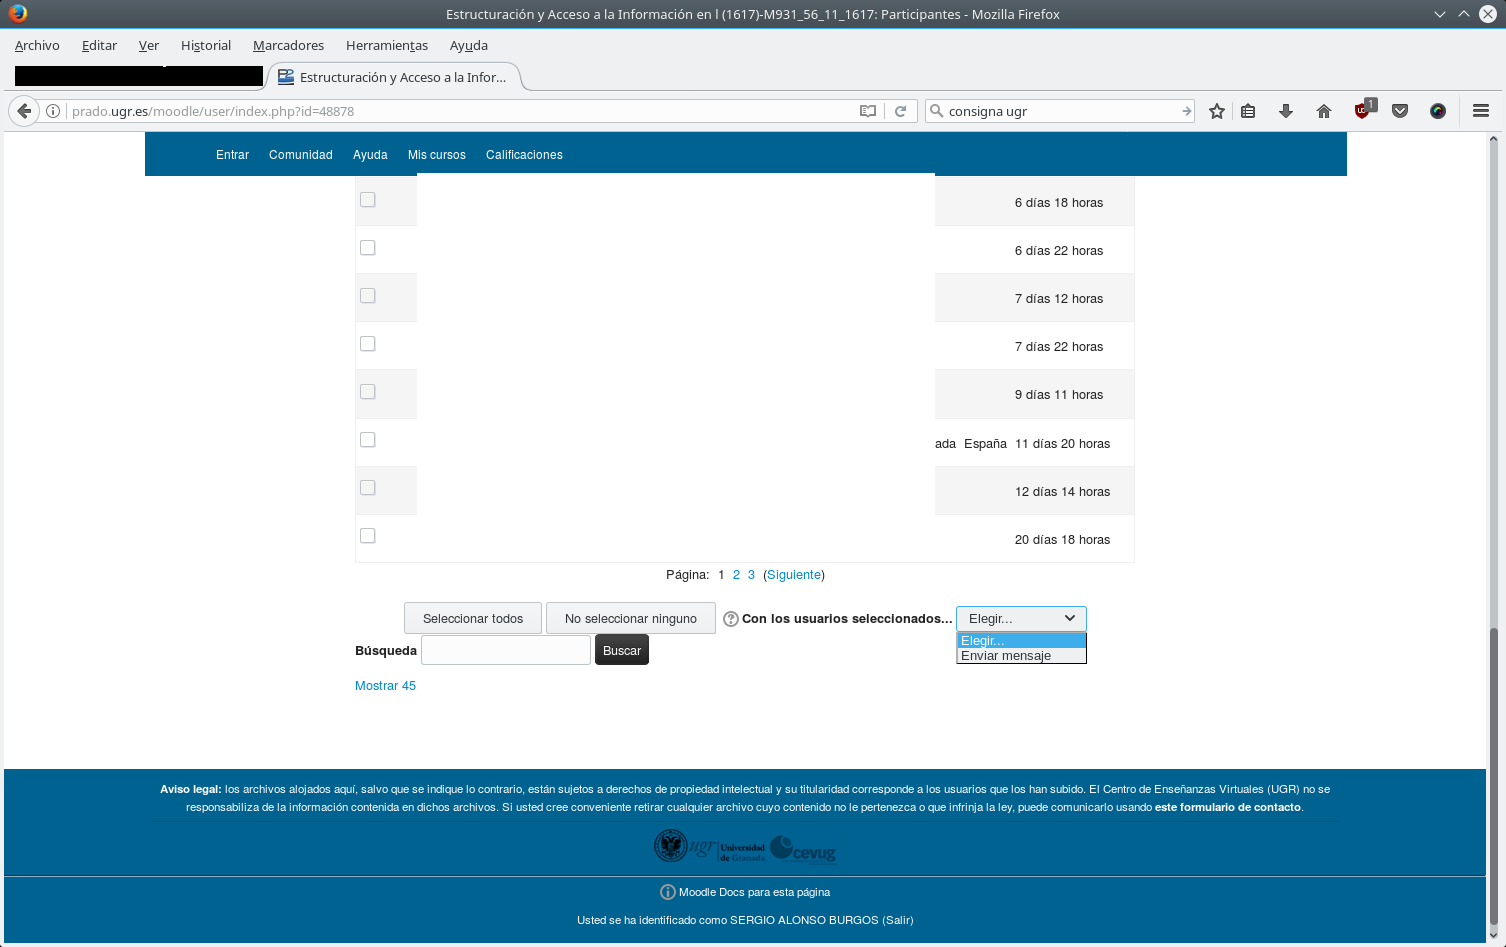
\includegraphics[width=0.8\textwidth]{../screenshots/pantallazoPradoenviarMensaje}
\caption{Vista principal del clon de Prado}
\label{fig:pantallazoPradoenviarMensaje}
\end{figure}

\begin{figure}[h!]
\centering
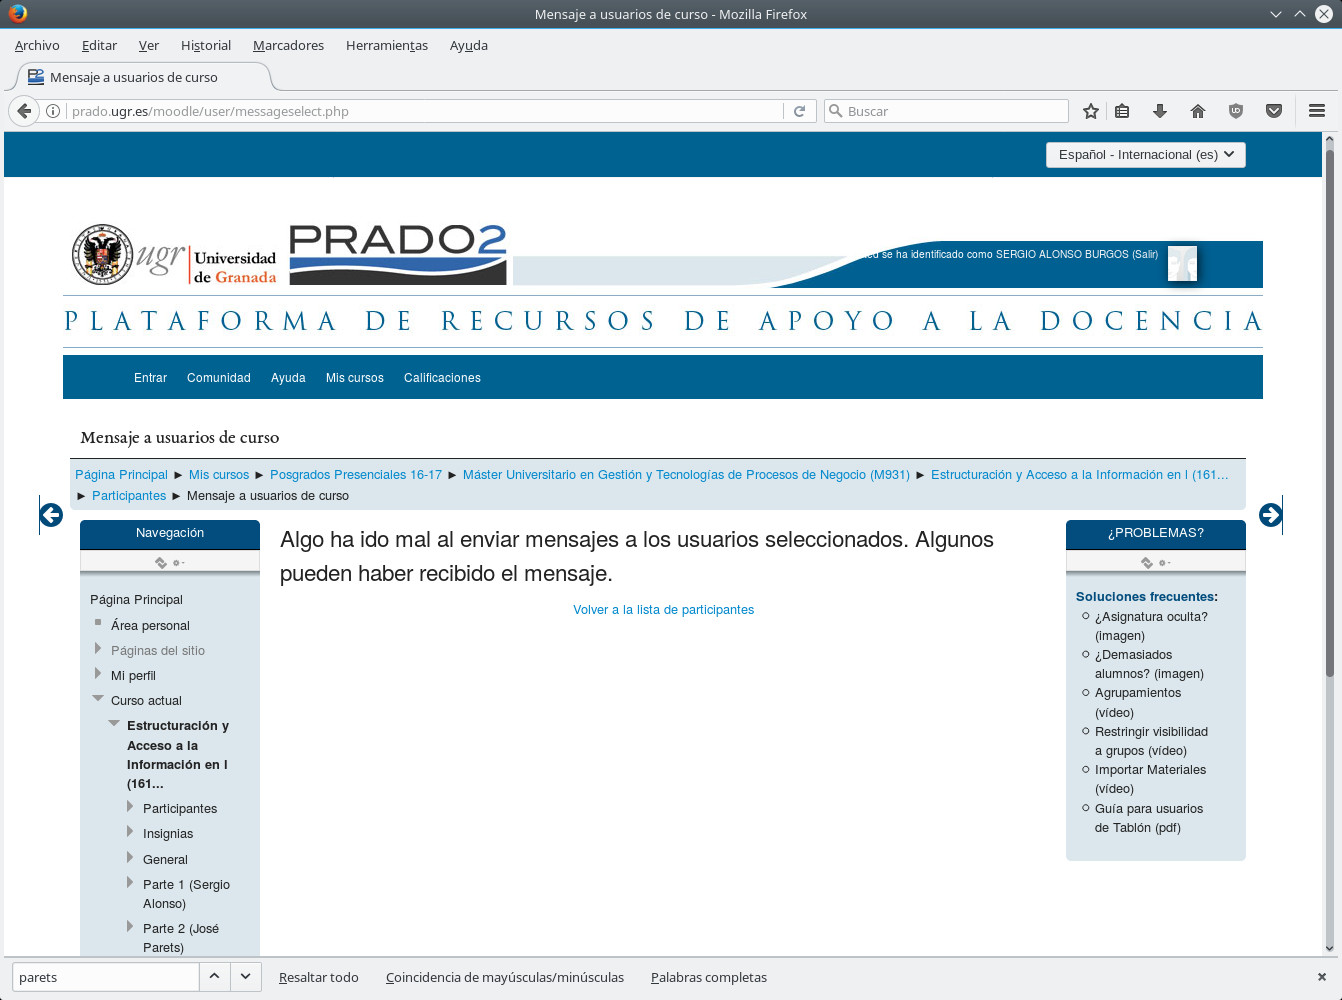
\includegraphics[width=0.8\textwidth]{../screenshots/pantallazoPradoMensaje2}
\caption{Error mostrado al enviar mensaje}
\label{fig:pantallazoPradoMensaje2}
\end{figure}


\item No hay una opción sencilla para crear un listado con los alumnos de cada grupo. Esta  opción puede ser interesante, por ejemplo, para imprimir y llevar un control manual.

\item En la vista de grupos, los nombres salen cortados y además sólo aparecen los apellidos de los alumnos pero no sus nombres. Esto es un problema para alumnos con los mismos apellidos, además no se puede reordenar de ninguna forma.

\item El menú superior donde aparecen las opciones ``Entrar'', ``Comunidad'', `Ayuda'' y ``Mis cursos'' no tiene un sentido claro: La opción ``Entrar` aparece siempre aunque la sesión esté iniciada, el menú ``Comunidad` está accesible más adelante y no tiene una importancia tal y como aparecer en la parte superior, el menú ``Ayuda'' nos lleva a una pagina externa del CEVUG para abrir un ticket y el menú ``Mis Cursos'' lleva a una vista que no es la misma que la de la página principal de \textit{Prado2}.

\item La búsqueda de cursos suele tardar demasiado en responder.

\item Las novedades del curso y del sitio no parecen tener ninguna utilidad.

\item Aunque se configuren agrupamientos de alumnos, los mismos luego no se pueden utilizar para nada. De hecho, no sirven ni para hacer un listado de alumnos por grupo.

\item No se entiende la utilidad del foro privado, quizá esa opción no debería estar. Igual sucede con las insignias.

\item El árbol de navegación lateral es confuso y la estructura de bloques no es consistente. Además, en cada cambio de página se vuelve a mostrar la vista por defecto. Se puede hacer la prueba mostrando el bloque ``Calendario'' de la parte derecha y haciendo click en cambiar de mes, vemos que se recarga la pagina ocultando de nuevo el bloque ``Calendario''. Al entrar en la página aparecen a la izquierda cuatro bloques diferenciados: ``Enlaces'', ``Menú Principal'', ``Navegación'' y ``Administración'' pero, al entrar en cualquier opción, los dos primeros desaparecen.

\item En los listados no se puede ordenar por rol del usuario, por lo que los distintos profesores de una asignatura aparecen mezclados con los alumnos.

\item Aunque se oculten los bloques laterales con las flechas que hay para tal cometido, al recargar la página esos bloques vuelven a aparecer.

\item Si hago colapsar las columnas de navegación laterales (flechas izquierda y derecha), en cuanto hago click en otro enlace vuelven a aparecer. Esto obliga a estar colapsándolas todo el rato.

%\item Las herramientas de grupos/agrupamientos me han dado algo de trabajo. Creo que ya lo controlo, pero me da la sensación de que podrían ser más fáciles.

\item Al enviar un mensaje a un estudiante a través de \textit{Moodle}, no se puede poner un ``Asunto''. %Imagino que simplemente le sale en 'Asunto' el nombre de la asignatura, pero me gustaría poder poner algo más específico.

\item Aunque \textit{Moodle} preserve el anonimato en las respuestas de los cuestionarios, no preserva dicho anonimato en el ``registro de actividad''. Es decir, se puede saber quién ha respondido a la encuesta e incluso, si uno está pendiente de cada actualización del registro, saber quién es el autor de cada respuesta. Si una actividad se etiqueta como anónima, el acceso a la misma debería desaparecer del registro de actividad.

%\item Todos los cursos pongo un cuestionario de valoración de la asignatura que los estudiantes pueden responder anónimamente. Moodle preserva el anonimato en las respuestas, pero no en el 'registro de actividad'. Es decir, se puede saber quiénes respondieron al cuestionario e incluso, si uno estuviera muy pendiente de cada actualización de respuestas, quién es responsable de cada respuesta. Creo que cuando una actividad se etiqueta como anónima, el acceso a la misma debería desaparecer del registro de actividad.

\item Al poner una fecha de inicio y fin de una actividad, debería aparecer por defecto el año en que estamos. Un usuario nos contó que en una ocasión, la actividad se daba por cerrada un año antes.

%\item No sé de quién depende esto pero, por favor, que aparezcan en moodle todos los estudiantes matriculados en la asignatura, y sólo ellos.

\item Hemos notado también un malestar general con los estudiantes que inscritos automáticamente en las asignaturas. En algunos casos, se inscriben estudiantes que no están matriculados y en otros, alumnos matriculados no aparecen inscritos en sus asignaturas.

%\item Es una locura el tema de la matrícula de los estudiantes; me han escrito estudiantes para decirme que a pesar de estar en otro curso y no haberse matriculado nunca en mi asignatura, aparecen y, por tanto, les llegan los mensajes y tienen acceso a la plataforma. Por el contrario, hay muchos estudiantes que tengo que matricular manualmente porque, a pesar de estar en mi grupo, no aparecen!!! 

\item El problema de la adjudicación de grupos de alumnos en el master de educación. Aparecen los alumnos de todas las especialidades en la misma asignatura y todos los profesores pueden subir o borrar recursos de la plataforma, aunque no sean profesores de ese grupo en concreto.

% MARTA: llego hasta aquí revisando. Después sigo :P

\item Las sesiones de usuario (sobre todo cuando se visualiza desde el smartphone) se mantienen de una forma muy rara, ha habido veces que se ha cerrado sin motivo alguno y hay que volver a iniciar sesión. Adicionalmente, se debería habilitar un botón para recordar la sesión.

\item La usabilidad deja mucho que desear, la plataforma no es nada intuitiva.

\item En general los profesores no saben utilizar la opción de elegir grupo, optando por pasar una hoja en papel y que cada uno se apunte donde quiera.

\item No se muestra con claridad los archivos nuevos o novedades en general, de forma que el usuario tiene que estar buscando qué ha visto ya y qué no.

\item La plataforma funciona con lentitud y las caídas son muy frecuentes, en ocasiones en horas críticas para la entrega de ejercicios (entre las 22:00 y las 00:00)

\item La plataforma en general carece de estilo y orden alguno, las cosas están por medio sin una estructura de calidad.

\item Estaba haciendo unas cosas del Departamento y he tenido que acceder a Prado. Entonces he caído en la cuenta de otras dos cosas que no tenía anotadas y para las que no hay opción directa en Prado: poner el horario de teoría y prácticas de la asignatura y poner el horario de tutorías del profesorado implicado (tampoco sale en la parte personal). En general, los datos de la asignatura (incluso objetivos, temario de teoría y temario de prácticas) y los del profesorado que la imparte, brillan por su ausencia. Dos puntos más, y gordos, a favor de SWAD.

\item Todas esas cosas las he podido poner en Prado, pero en un archivo en pdf que yo me he creado con la presentación de la asignatura.
\end{enumerate}

\section{Encuesta a los usuarios}

Durante el tiempo que estuvo operativa la encuesta recibimos un total de 617 respuestas, como se puede apreciar en el gráfico la mayor parte de las respuestas se obtuvieron tras las peticiones de participación via e-mail.

    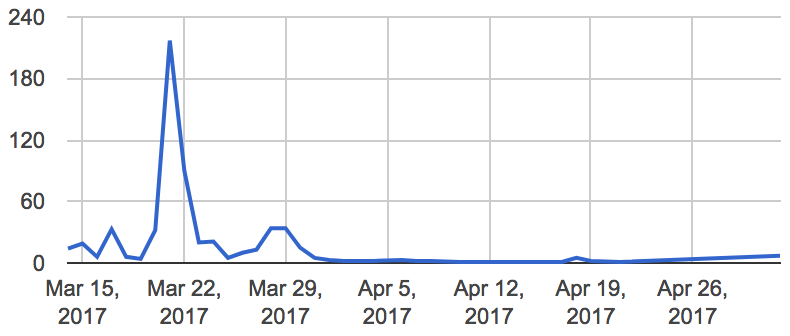
\includegraphics[width=0.8\textwidth]{../charts/00_fecha}
 	

\begin{enumerate}

  \item \textbf{Selección del tipo de usuario} 
  
  La mayor parte de los encuestados han sido alumnos superando el 83\% del ratio, casi un 15\% han sido profesores y el resto otro tipo de usuarios como pueden  ser estudiantes de doctorado y antiguos alumnos.
  
  
	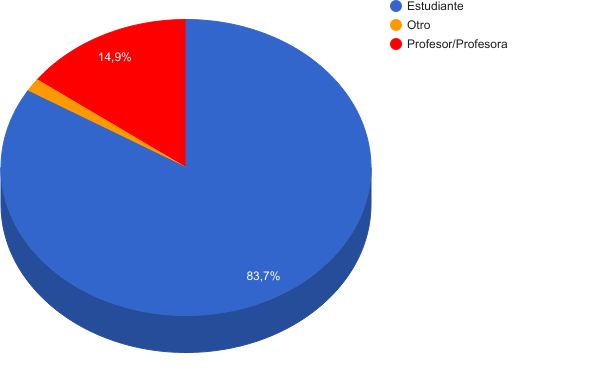
\includegraphics[width=0.8\textwidth]{../charts/01_esusted}
  

  \item \textbf{Selección de la titulación} 
  
  Debido al carácter de este proyecto esperábamos una mayoría de participantes de estudiantes de carreras impartidas en la ETSIIT como pueden ser el Grado de Ingeniería Informática, el Grado de Ingeniería en Tecnologías de Telecomunicación y el Doble Grado en Ingeniería Informática y Matemáticas, pero nos ha sorprendido ver la alta participación de otros estudios como pueden ser Administración y Dirección de Empresas, Medicina y Psicología por nombrar las titulaciones mas representativos de las casi 70 participantes.
  
  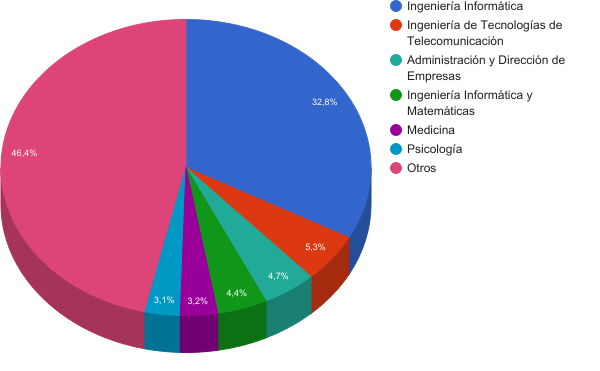
\includegraphics[width=0.8\textwidth]{../charts/02_titulacion}


  \item \textbf{¿Con qué periodicidad accede a Prado2?} 
  
  La mayoría de los usuarios acceden a la plataforma con mucha frecuencia lo que refuerza nuestra opinión de que por un lado se tiene que optimizar la plataforma para que esos accesos sean lo mas breves y satisfactorios posibles, muchos de estos accesos se reducirían si el sistema notificara vía e-mail o a través de un aplicación móvil si hay alguna actividad nueva en mis cursos. De igual manera se reduciría carga en el servidor si se supiera que los documentos subidos por el profesor no han subido cambios y no hubiera que descargarlos de nuevo para comprobarlo manualmente.

  
  
  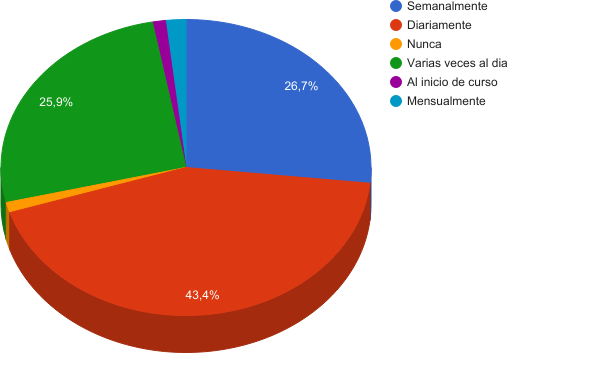
\includegraphics[width=0.8\textwidth]{../charts/03_periodicidad}

  
  \item \textbf{Califique las siguientes opciones según sus necesidades} 

Lo que mas piden los usuarios con diferencia es poder ver las calificaciones en Prado2, eso nos lo han hecho saber tanto en la opción de la encuesta como varios comentarios personales. Por otra parte muchos profesores nos han hecho saber que con el sistema actual tiene que hacer el trabajo por duplicado introduciendo las calificaciones en Prado2 y por otro lado en el sistema de actas de la UGR, cuando sería muchos mas cómodo poder generar en prado algún tipo de fichero CSV que les permitiera entregar las actas.

  
Casi todos los usuarios coinciden en que es vital el acceso desde dispositivos móviles, ya sea mediante una aplicación para smartphone como desde una web con un diseño adaptado a móviles ya que aunque el diseño actual tiene partes que si se adaptan para móviles no es apto para su uso ya que se hace inmanejable.

Los usuarios también creen necesario un sistema de mensajería interna para la comunicación entre profesores y alumnos.

En cambio, las opciones de Insignias, Blogs y Estadísticas no parecen ser vitales y de hecho mucha gente nos ha preguntado que utilidad tienen las Insginias pues no saben para que sirven.

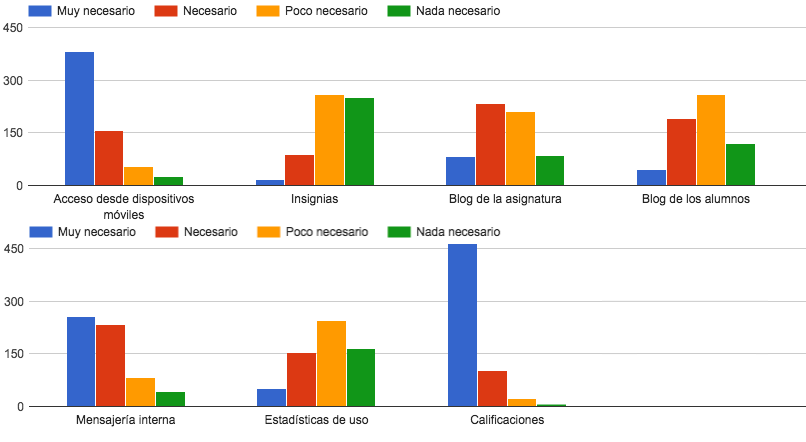
\includegraphics[width=0.8\textwidth]{../charts/04_califique} 

  \item \textbf{Actividades y recursos} 

En cuanto a actividades podemos ver que al igual que en las instalaciones de moodle de otras universidades las opciones mas usadas son las de agregar tareas y archivos, hay que tener en cuenta que hay actividades que básicamente son similares a agregar archivo, como puede ser carpeta, documento, página y libro. 

Aunque moodle tiene actividades que podrían ser muy útiles, como pueden ser los paquetes SCORM e IMS, el desconocimiento y/o la falta de formación hace que la gente ignore para que sirven.

Igual pasa con algunas tareas específicas creadas para la UGR como pueden ser las clases grabadas (GA3), aunque si hay tareas que son necesarias aunque tengan muy poca utilización como pueden ser la selección de grupo de prácticas al inicio del curso y el control de asistencia.


\begin{figure}[H]
\centering
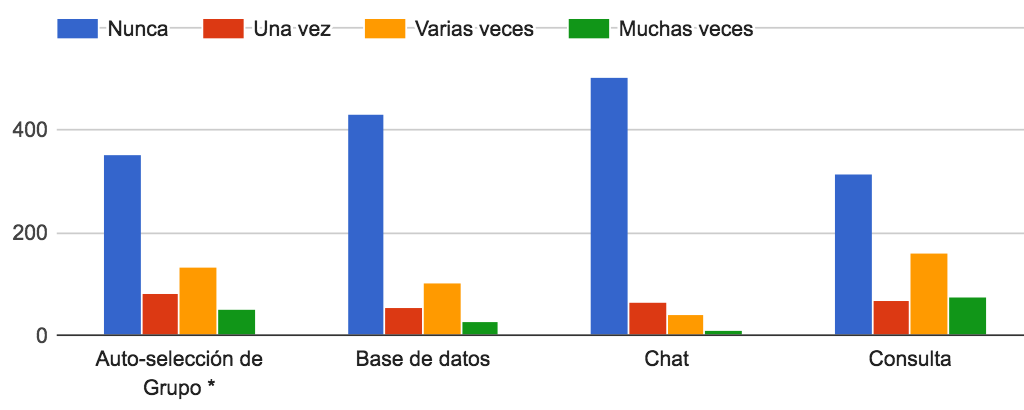
\includegraphics[width=0.8\textwidth]{../charts/05_actividades_01} 
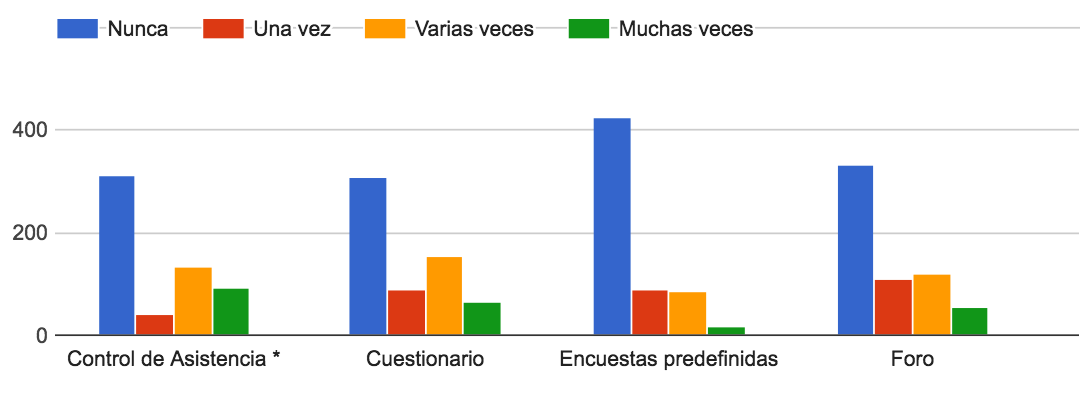
\includegraphics[width=0.8\textwidth]{../charts/05_actividades_02} 
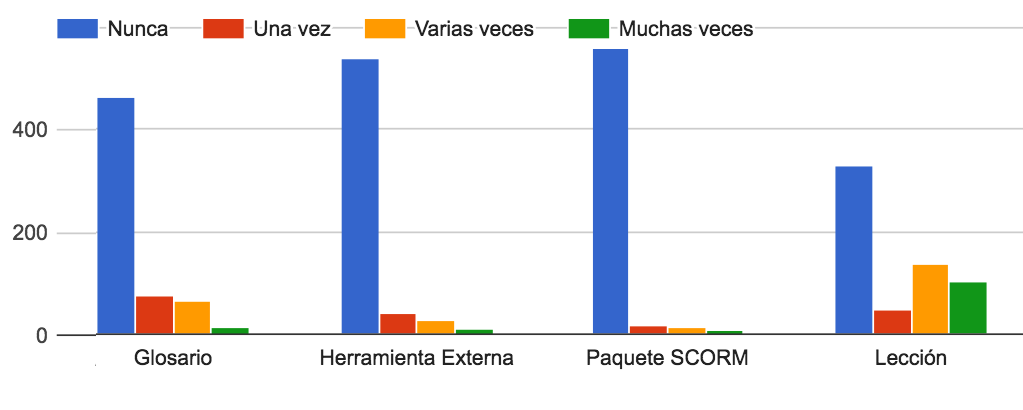
\includegraphics[width=0.8\textwidth]{../charts/05_actividades_03} 
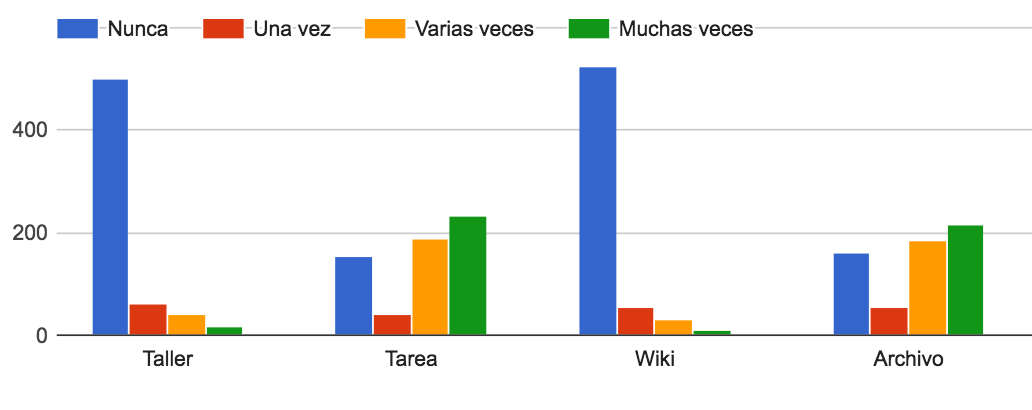
\includegraphics[width=0.8\textwidth]{../charts/05_actividades_04} 
\end{figure}
\begin{figure}[H]
\centering
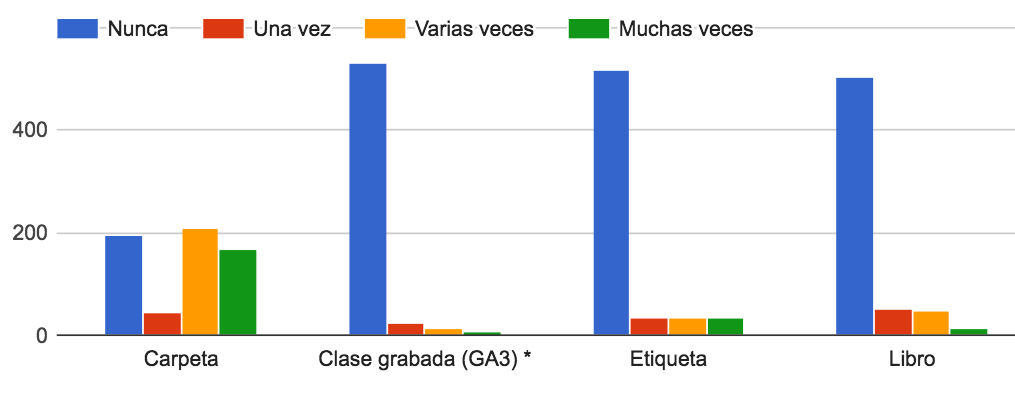
\includegraphics[width=0.8\textwidth]{../charts/05_actividades_05} 
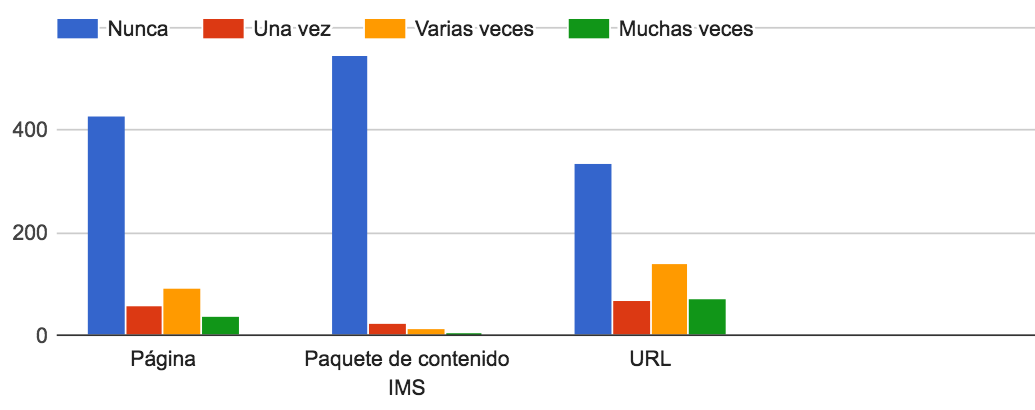
\includegraphics[width=0.8\textwidth]{../charts/05_actividades_06} 

\end{figure}

  \item \textbf{¿Cómo calificaría Prado2?}
  
  
A la hora de calificar prado han la mayoría de los usuarios han otorgado aprobado lo cual es una buena señal, aunque se piense que hay un descontento generalizado la gente entiende que una plataforma puede tener problemas y simplemente espera que se solucionen. Aun con el aprobado general, los usuarios si que encuentran en gran medida muy deficiente la usabilidad de la plataforma. En cambio el sentimiento general es el de que la plataforma es segura.

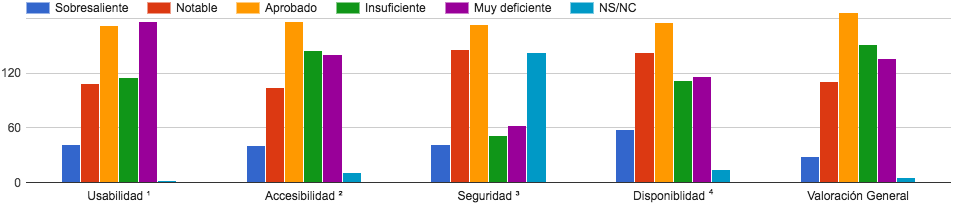
\includegraphics[width=0.8\textwidth]{../charts/06_calificaria}


  \item \textbf{¿Con cúales de las siguientes plataformas de la UGR ha trabajado?} 

Aquí hay tres ganadores claves, y son evidentemente las plataformas que mas se han usado en todo el ámbito UGR como pueden ser el Tablon de Docencia, SWAD y el propio Prado2, luego encontramos plataformas usadas solo en la ETSIIT como pueden ser Tutor y DECSAI y algunos otros como el antiguo moodle del CEVUG y Ágora que es otra instalación de moodle utilizada en la facultad de Psicología.

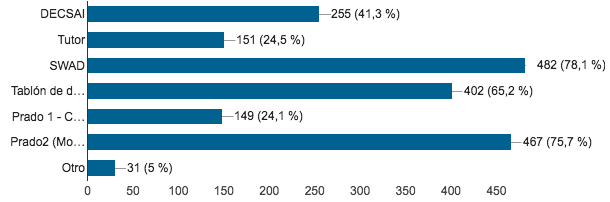
\includegraphics[width=0.8\textwidth]{../charts/07_plataformastrabajado}

  \item \textbf{De las siguientes plataformas de la UGR ¿Cuál prefiere?} 

A la hora de establecer la plataforma favorita está clara la prevalencia de SWAD ya que es una plataforma potente y con muchos años de uso aunque Prado2 también tiene una buena acogida y mas teniendo en cuenta la sensación de descontento generalizado que percibíamos antes de comenzar este proyecto, esto quiere decir que tampoco se va por mal camino con la plataforma actual. Curioso cuanto menos que el Tablón de Docencia, una arcaica plataforma utilizada en la UGR sigue teniendo sus partidarios pero como ya hemos comentado anteriormente una de las cosas con las que más cuesta lidiar en cuanto a la usabilidad es la resistencia de los usuarios al cambio, aunque este sea a mejor.

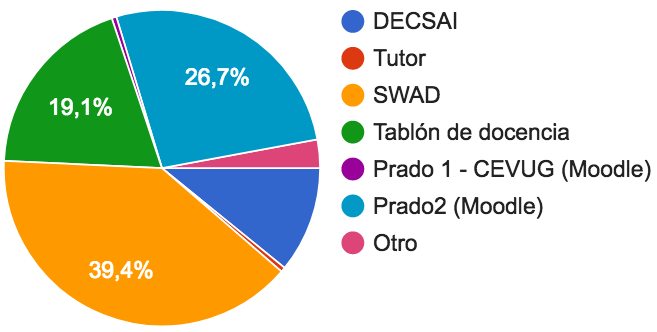
\includegraphics[width=0.8\textwidth]{../charts/08_plataformas_prefiere} 

  \item \textbf{¿Ha encontrado algún error que debería ser subsanado en Prado2?} 

Esta pregunta al ser de entrada libre se adjuntará en el listado en bruto de respuestas   

  \item \textbf{Indique cuál es la funcionalidad que más le gusta de Prado2} 

Esta pregunta al ser de entrada libre se adjuntará en el listado en bruto de respuestas

  \item \textbf{Comentarios adicionales} 
  
Esta pregunta al ser de entrada libre se adjuntará en el anexo VI
  
\end{enumerate}


\section{Análisis de registros propios de la plataforma}

Tras analizar los registros proporcionados por el CEVUG de los años 2015 y 2016 vemos que los resultados de la encuesta cuadran con los mismos.

No hemos analizado la muestra que nos proporcionaron de 2014 ya que fue en el curso 2015-2016 como se puede apreciar en la figura \ref{fig:distintonumerousuarios_2015}.

Lo primero a destacar son el notable incremento de peticiones del año 2015 al año 2016 que se puede apreciar en la tabla de la figura \ref{table:sumarioregistros}.

\begin{table}[H]
\centering
\begin{tabular}{|l|r|r|}
\hline
\textbf{Año}        & \textbf{2015}	& \textbf{2016} 		\\ \hline
Número de registros & 3.119.094     	& 20.243.312			\\ \hline
Usuarios únicos     & 19.448        & 51.283				\\ \hline
IPs distintas       & 115.349       & 370.580			\\ \hline
Cursos              & 1.266         & 8.414				\\ \hline
Módulos             & 32            & 32					\\ \hline
\end{tabular}
\caption{Sumario de los registros de los años 2015 y 2016}
\label{table:sumarioregistros}
\end{table}

En las figuras de la \ref{fig:actividadtotal_2015} a la \ref{fig:frecuenciausuarios_2016} podemos ver como el grueso de la actividad se lo llevan unos pocos usuarios, es decir, la inmensa mayoría interactúa muy poco con la plataforma. Presuponemos que este grueso de actividad pertenece tanto a los administradores como a un reducido círculo de profesores, hay que tener en cuenta que los logs registran cada click en alguna sección de Prado.

\begin{figure}[H]
\centering
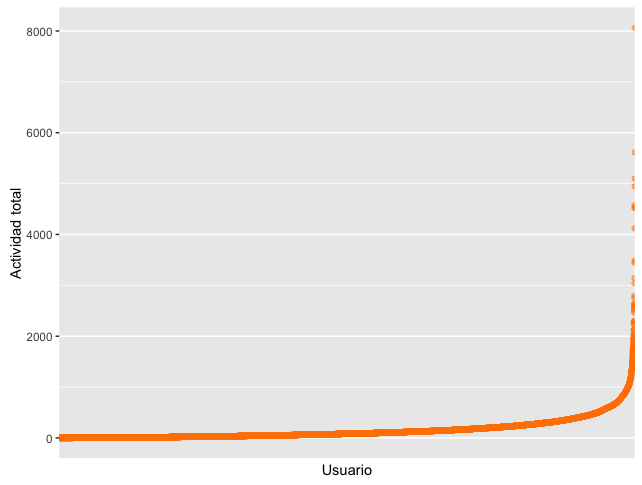
\includegraphics[width=0.9\textwidth]{../r/actividadtotal_2015}
\caption{Actividad total en 2015}
\label{fig:actividadtotal_2015}
\end{figure}

\begin{figure}[H]
\centering
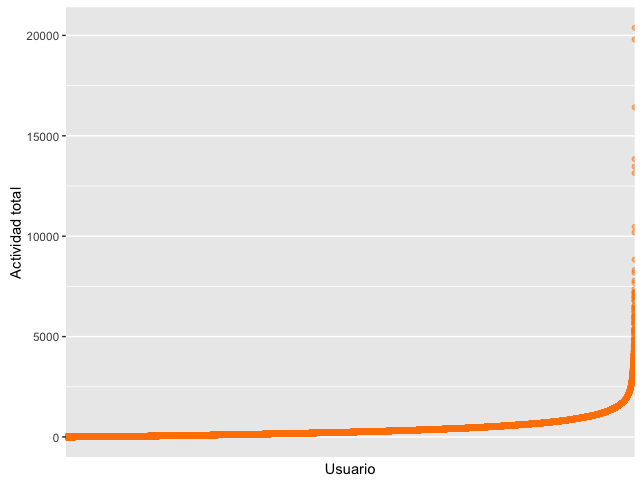
\includegraphics[width=0.9\textwidth]{../r/actividadtotal_2016}
\caption{Actividad total en 2016}
\label{fig:actividadtotal_2016}
\end{figure}

\begin{figure}[H]
\centering
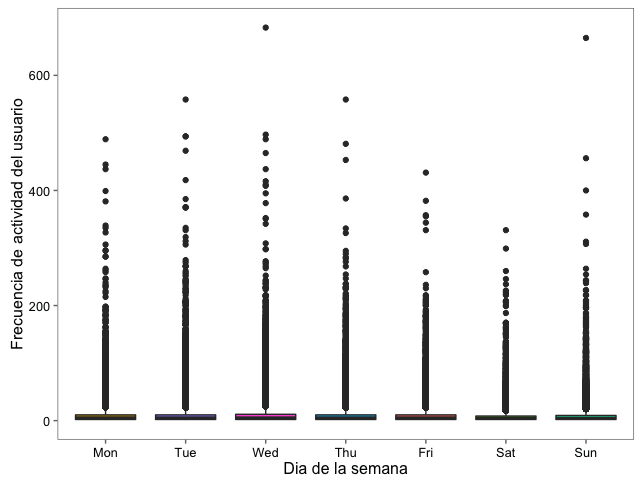
\includegraphics[width=0.9\textwidth]{../r/frecuenciaactividadusuario_2015}
\caption{Frecuencia de actividad de los usuarios en 2015}
\label{fig:frecuenciaactividadusuario_2015}
\end{figure}

\begin{figure}[H]
\centering
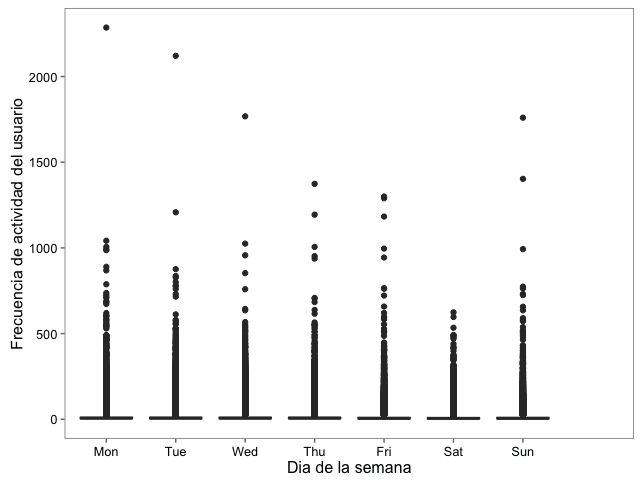
\includegraphics[width=0.9\textwidth]{../r/frecuenciaactividadusuario_2016}
\caption{Frecuencia de actividad de los usuarios en 2016}
\label{fig:frecuenciaactividadusuario_2016}
\end{figure}


\begin{figure}[H]
\centering
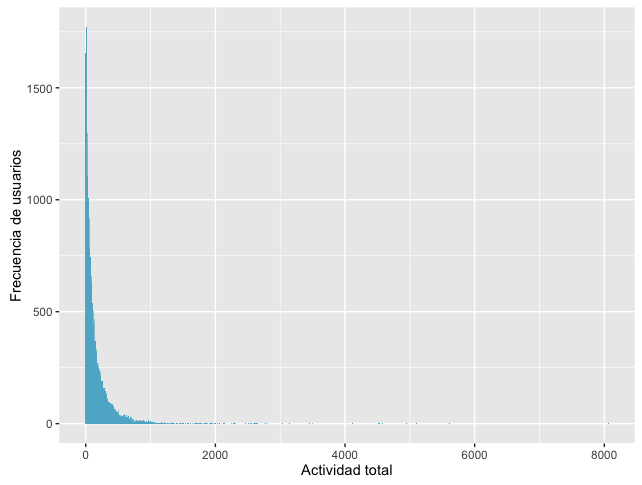
\includegraphics[width=0.9\textwidth]{../r/frecuenciausuarios_2015}
\caption{Frecuencia de usuarios en 2015}
\label{fig:frecuenciausuarios_2015}
\end{figure}


\begin{figure}[H]
\centering
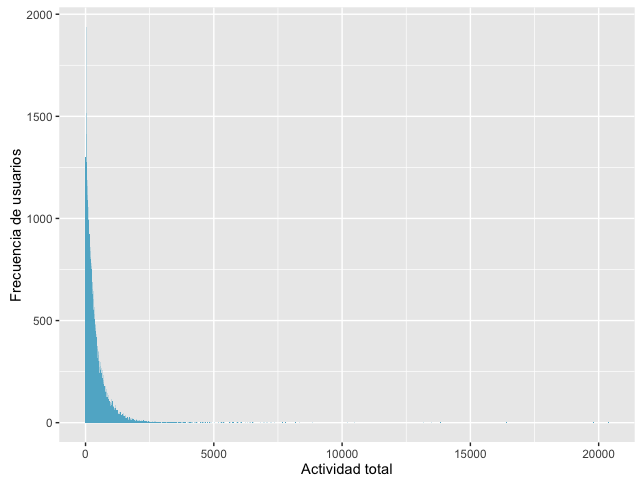
\includegraphics[width=0.9\textwidth]{../r/frecuenciausuarios_2016}
\caption{Frecuencia de usuarios en 2016}
\label{fig:frecuenciausuarios_2016}
\end{figure}

También vemos en las figuras \ref{fig:distintonumerousuarios_2015} y \ref{fig:distintonumerousuarios_2016} como los usuarios comenzaron a hacer uso de la plataforma en Septiembre de 2015 que es cuando oficialmente se comenzó a utilizar Prado.



\begin{figure}[H]
\centering
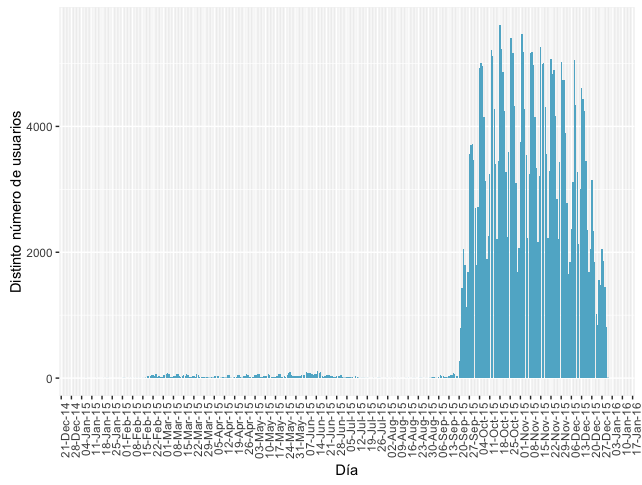
\includegraphics[width=0.9\textwidth]{../r/distintonumerousuarios_2015}
\caption{Interacciones de usuarios únicos en 2015}
\label{fig:distintonumerousuarios_2015}
\end{figure}

\begin{figure}[H]
\centering
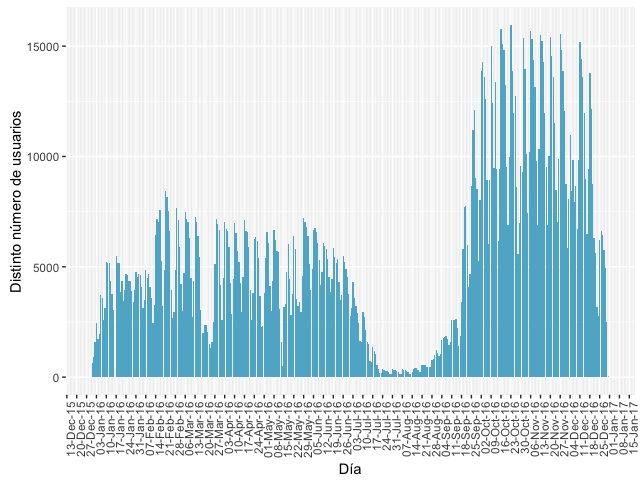
\includegraphics[width=0.9\textwidth]{../r/distintonumerousuarios_2016}
\caption{Interacciones de usuarios únicos en 2016}
\label{fig:distintonumerousuarios_2016}
\end{figure}


En las figuras \ref{fig:frecuenciaactividaddiaria_2015} y \ref{fig:frecuenciaactividaddiaria_2016} se percibe como la mayoría de los usuarios utilizan la plataforma en las horas lectivas, descenciendo la utilización como es evidente los fines de semana, también nos sirve para ver como la madrugada es la hora ideal para realizar cambios en la plataforma pues el a esas horas casi no hay usuarios usando Prado.

\begin{figure}[H]
\centering
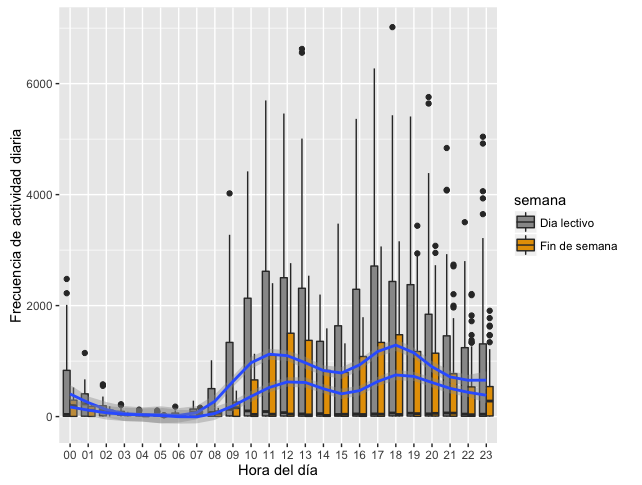
\includegraphics[width=0.9\textwidth]{../r/frecuenciaactividaddiaria_2015}
\caption{Frecuencia de actividad diaria en 2015}
\label{fig:frecuenciaactividaddiaria_2015}
\end{figure}

\begin{figure}[H]
\centering
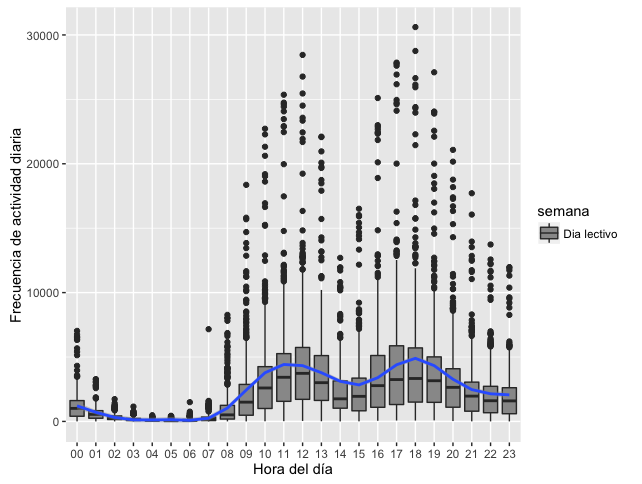
\includegraphics[width=0.9\textwidth]{../r/frecuenciaactividaddiaria_2016}
\caption{Frecuencia de actividad diaria en 2016}
\label{fig:frecuenciaactividaddiaria_2016}
\end{figure}


En cuanto a las actividades podemos ver en las figuras \ref{fig:usoactividades_2015} y \ref{fig:usoactividades_2016} así como en la tabla \ref{table:usoactividades_2015} que tal y como concluimos en la encuesta la gran mayoría de las actividades disponibles en moodle no tienen apenas uso. Hay que destacar que la actividad 'course' se refiere a cada vez que un usuario ve contenido de un curso acaparando la mitad de las interacciones, la actividad 'user' se crea cada vez que se ve el perfil de un usuario o profesor y la actividad 'assign' es para uso interno de moodle. Exceptuando estos tres casos vemos como las mas usados los cuestionarios y los archivos.

\begin{figure}[H]
\centering
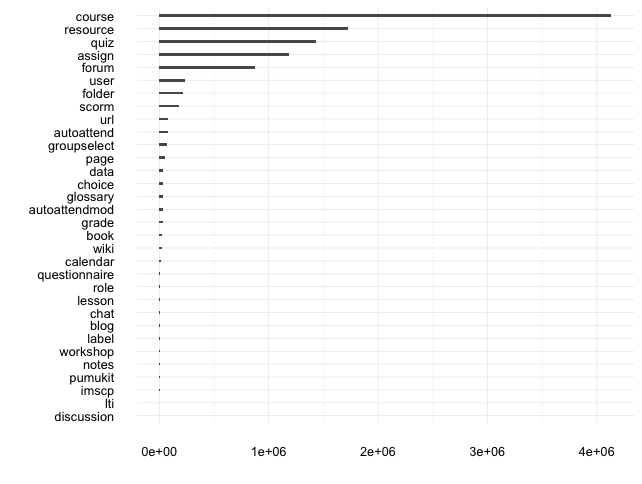
\includegraphics[width=0.9\textwidth]{../r/usoactividades_2015}
\caption{Uso de actividades en 2015}
\label{fig:usoactividades_2015}
\end{figure}

\begin{figure}[H]
\centering
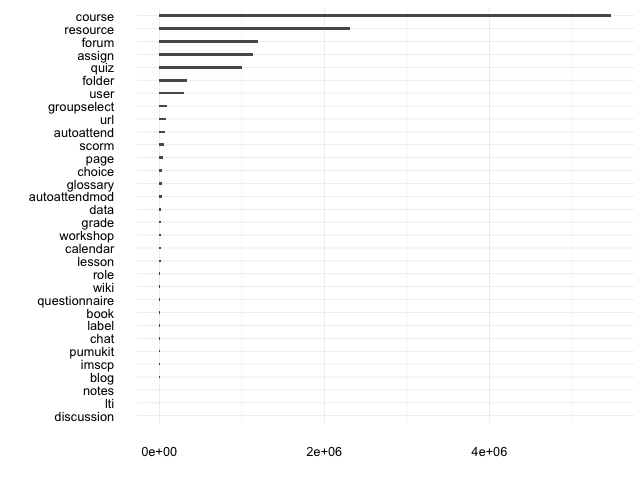
\includegraphics[width=0.9\textwidth]{../r/usoactividades_2016}
\caption{Uso de actividades en 2016}
\label{fig:usoactividades_2016}
\end{figure}

\begin{table}[H]
\centering
\begin{tabular}{|l|r|r|}
\hline
\textbf{Módulo} & \textbf{2015} & \textbf{2016} \\ \hline
course          & 1204043       & 8631749       \\ \hline
quiz            & 480975        & 1967505       \\ \hline
resource        & 464898        & 3680181       \\ \hline
assign          & 381096        & 1985887       \\ \hline
forum           & 233528        & 1905834       \\ \hline
user            & 81118         & 473303        \\ \hline
folder          & 65733         & 499643        \\ \hline
scorm           & 33459         & 205890        \\ \hline
url             & 25720         & 139415        \\ \hline
autoattend      & 25530         & 112115        \\ \hline
groupselect     & 25518         & 132941        \\ \hline
page            & 22382         & 79816         \\ \hline
choice          & 11514         & 58419         \\ \hline
autoattendmod   & 11020         & 47220         \\ \hline
glossary        & 9244          & 50541         \\ \hline
lesson          & 6702          & 14140         \\ \hline
wiki            & 6040          & 26199         \\ \hline
calendar        & 4988          & 23273         \\ \hline
questionnaire   & 4961          & 13241         \\ \hline
data            & 4525          & 51868         \\ \hline
book            & 4485          & 31140         \\ \hline
grade           & 2809          & 46357         \\ \hline
role            & 2306          & 16770         \\ \hline
blog            & 1665          & 4616          \\ \hline
chat            & 1351          & 7267          \\ \hline
label           & 1282          & 7014          \\ \hline
notes           & 1174          & 3362          \\ \hline
imscp           & 396           & 2789          \\ \hline
pumukit         & 305           & 4717          \\ \hline
discussion      & 118           & 344           \\ \hline
workshop        & 117           & 18395         \\ \hline
lti             & 92            & 1357          \\ \hline
\end{tabular}
\caption{Tabla detallada del uso de actividades en 2015 y 2016}
\label{table:usoactividades_2015}
\end{table}


\section{Análisis de usabilidad de la plataforma}

Analizamos la plataforma como un usuario normal para ver con que problemas se podía encontrar a la hora de usar Prado. Nos hemos centrado en los problemas de usabilidad con fácil solución y que harían la experiencia de usuario mucho más placentera.

\bigskip
En nuestro análisis hemos encontrado los siguientes problemas:

\begin{itemize}

\item Aparece la información para iniciar sesión en la cabecera y en el pié de la página, esto es redundante, debería aparecer solo en la cabecera.
\item El selector de idioma ocupa una gran parte de la pantalla siendo un elemento de uso poco común. De hecho como veremos más adelante la traducción al inglés brilla por su ausencia, lo ideal en estos casos es colocar los enlaces para cambiar el idioma en el pié de página. Hay que tener en cuenta que la plataforma detecta el idioma del navegador para seleccionar Español o Inglés. Además debería poner 'Castellano' en lugar de 'Español - Internacional'.
\item El título 'PLATAFORMA DE RECURSOS DE APOYO A LA DOCENCIA' no debería aparecer como una imagen, ya que además de no estar traducida hace que no todos los dispositivos la muestren bien al ser una imagen demasiado ancha.
\item La ventana de login muestra una imagen con la ruta https hacia el proveedor de identidad del CSIRC, un poco mas abajo nos encontramos un botón con la misma ruta pero con http. El IDP automáticamente redirige a https, este botón debería ocultarse. El acceso para administradores también debería ocultarse.
\item Debajo del banner de título aparece un menú con fondo azul en el que siempre aparece la opción 'Entrar' aunque ya hayamos iniciado la sesión en la plataforma.
\item La opción 'Comunidad' no tiene un uso tan importante como para aparecer ahí, quizá debería estar como un enlace en el pie. Además, podemos acceder al mismo desde el panel lateral.
\item La opción 'Ayuda' lleva a una página externa del CEVUG para solicitar asistencia, al tener un diseño distinto debería abrirse en una ventana nueva.
\item Con la sesión iniciada se muestran los cursos del alumno, pero al haber cursos con el mismo nombre hay que ir probando uno a uno con lo cual esta opción tampoco tiene utilidad.
\item Si se está dentro de un curso también vemos la opción 'Calificaciones', esta opción se puede ver desde el panel lateral y teniendo en cuenta que la mayoría de los profesores no ponen las calificaciones en prado quizá esta opción debería ocultarse.
\item En resumidas cuentas, este menú superior se podría ocultar sin ningún tipo de problema, ganando muchísimo espacio en la pantalla.
\item El banner central de información acapara toda la atención obligando al usuario a desplazarse para ver la información de los cursos que quiere ver. Dicho banner no muestra información útil con lo que quizá merecería quitarlo o por lo menos darle la opción a los usuarios de ocultarlo.
\item Aunque se permite ocultar los paneles laterales al recargar la página se vuelven a mostrar, debería memorizarse el estado seleccionado.
\item Al desplegar las secciones de cada panel lateral ocurre lo mismo que al ocultarlos, no se recuerda cual se tenía abierto. Esto resulta particularmente molesto al hacer uso del calendario en el panel derecho, pues al cambiar de mes se recarga la página ocultando la sección.
\item El panel de la izquierda no sigue un orden lógico, según se va navegando por la página tiene entre 2 y 4 secciones principales aunque contenga la misma información. Pasa lo mismo en el derecho al entrar en una asignatura.
\item El panel derecho muestra una sección de 'Problemas' con información para los profesores que los alumnos no deberían de ver.
\item Al ver nuestro perfil no debería mostrarse la opción 'Personalizar esta página' ya que esto es lo que se usa para editar los cursos. Esto lleva a confusión al usuario pues piensa que esta opción es para editar su perfil y no es así.
\item Las insignias deberían ocultarse pues no se están utilizando.
\item Hay diversas vistas diferentes de 'Mis cursos', lo cual es bastante confuso.
\item Una vez dentro de un curso el foro de novedades se debería ocultar por defecto a no ser que el profesor lo active.
\item En la vista principal de la asignatura, para ver los archivos hay que desplegar primero las diferentes opciones, quizá sería mejor mostrar un árbol para poder desplegarlo todo de una vez en lugar de uno en uno.
\item Al entregar una tarea muchas veces se olvida de enviar para calificación, lo ideal sería que por defecto al crear una tarea sea el envío automático para calificación.
\item No se puede ver si han habido cambios en los archivos subidos por el profesor, ni la fecha de subida ni ninguna información. De hecho, el nombre del archivo no tiene por qué coincidir con el texto que aparece en Prado, aumentando la confusión.
\item No se pueden descargar todos los archivos de una asignatura de golpe, hay que ir uno a uno.
\item Cuando un profesor está en modo edición puede agregar archivos de forma sencilla arrastrándolos sobre la ventana de cursos, pero la web no lo explica. En la plantilla por defecto de moodle si que sale una notificación informando de esta funcionalidad. Esto se debería mostrar ya que facilita mucho la tarea de subir archivos a la plataforma.
\item Cuando un profesor va a agregar una actividad el menú que sale es enorme, quizá se debería mostrar los mas utilizados, dejar el resto ocultos y permitir mostrarlo en una vista avanzada.
\item La vista de 'Todos los cursos' se debería ocultar, pues es imposible utilizar un desplegable con mas de 1000 opciones.
\item La vista 'Novedades del sitio' no muestra nada y al seleccionarla cambia de posición en el panel lateral, lo ideal sería ocultarla.
\item Se muestran varias asignaturas iguales, esto es confuso. Aunque internamente se creen para facilitar la administración lo ideal sería agruparlas en la misma vista para los alumnos.
\item El sistema de mensajería contiene un desplegable con la opción 'Enviar mensaje', para una sola opción sería mas sencillo un botón.

\end{itemize}

\section{Análisis de accesibilidad de la plataforma}

Los resultados de los análisis automáticos de accesibilidad de la página principal de Prado (ver figuras \ref{fig:tawdis}, \ref{fig:tenon} y \ref{fig:htmlcodesniffer}) indican que la plataforma tiene algunos puntos que corregir para cumplir con el estándar AA de accesibilidad. No se ha podido analizar de forma automática las páginas internas pues dichas herramientas no pueden acceder a la Plataforma porque hay que autentificarse. El resultado de dicho análisis automático es positivo pues la gran mayoría son pequeños detalles como asignación de etiquetas \texttt{alt}\footnote{Las etiquetas 'alt' se usan en las imágenes como “alternate text”, es decir, un texto que describe la imagen.} en imágenes. 

\bigskip
El test TAW nos indica que los colores de la plataforma pueden llegar a generar confusión y que sería adecuado un esquema de colores que permita distinguir de forma mas fácil la información importante así como las secciones principales.

\begin{figure}[H]
\centering
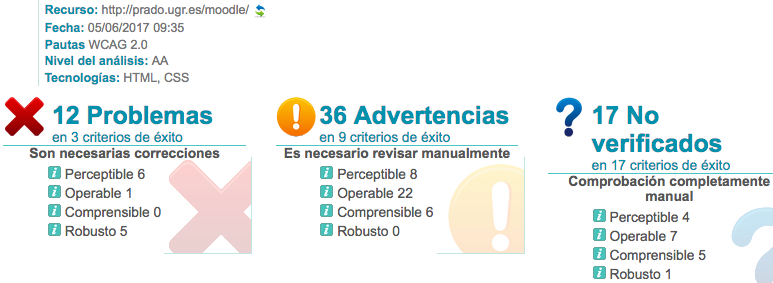
\includegraphics[width=0.9\textwidth]{../screenshots/tawdis}
\caption{Resultados de usabilidad con TAW}
\label{fig:tawdis}
\end{figure}

\begin{figure}[H]
\centering
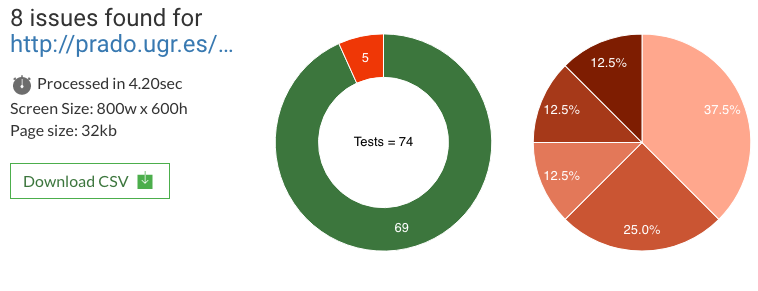
\includegraphics[width=0.8\textwidth]{../screenshots/tenon}
\caption{esultados de usabilidad con tenion.io}
\label{fig:tenon}
\end{figure}

\begin{figure}[H]
\centering
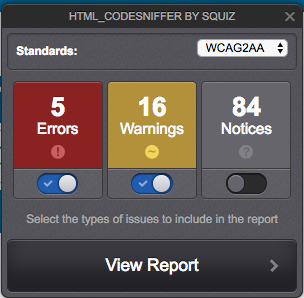
\includegraphics[width=0.6\textwidth]{../screenshots/htmlcodesniffer}
\caption{esultados de usabilidad con HTML CodeSniffer}
\label{fig:htmlcodesniffer}
\end{figure}


\bigskip
Aunque la plantilla utilizada es responsive\footnote{El diseño web responsive o adaptativo es una técnica de diseño web que busca la correcta visualización de una misma página en distintos dispositivos, desde ordenadores de escritorio a tablets y móviles}, los cambios realizados en la misma hacen que sea bastante incómoda de utilizar. Por un lado la vista principal debería mostrar mis cursos sin obligar a desplazarnos hacia abajo para obviar el mensaje de bienvenida. Al acceder a información como pueden ser calificaciones o entregas al no estar correctamente adaptado hay desplazarse horizontalmente y se pierde la noción de donde se está exactamente.

\bigskip
En la figura \ref{fig:capturamovil2} podemos ver como la ventana de inicio de sesión muestra una imagen que no está adaptada, con un botón mas abajo que realiza la misma función dando lugar a confusión, el acceso para personal técnico tampoco debería visualizarse y en la cabecera vemos como hay mucho espacio desperdiciado sin mostrar nada.

\bigskip
La plantilla tiene un menú 'hamburguesa' debajo de la imagen de perfil pero el ajuste realizado a la misma hace que se muestre parcialmente impidiendo su correcta utilización.


\begin{figure}[H]
\centering
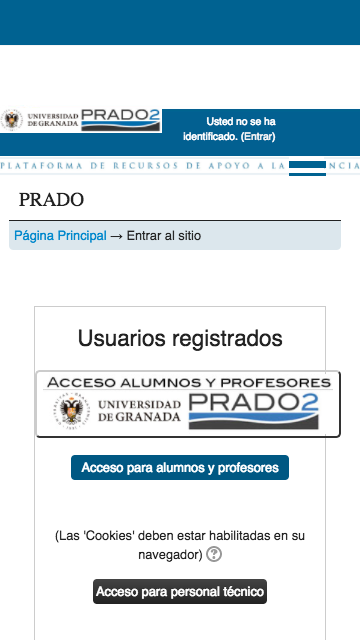
\includegraphics[width=0.5\textwidth]{../screenshots/capturamovil2}
\caption{Captura desde un teléfono móvil}
\label{fig:capturamovil2}
\end{figure}

\bigskip
La plataforma moodle está disponible en más de 100 idiomas pero en Prado se ha optado por habilitar castellano e inglés. El problema es que gran parte del contenido añadido a la plantilla, la ayuda y la información de los cursos se ha introducido de forma forzada en castellano con lo que el uso en inglés de la plataforma es prácticamente imposible. Varios alumnos de intercambio nos han hecho llegar sus quejas a la hora de manejarse en la plataforma, ya que no entienden que seleccionando la opción de idioma inglés la mayor parte de la interfaz y el contenido aparezca en castellano, creándoles confusión ya que muchos desconocen el castellano.

\bigskip
Si un usuario selecciona el idioma inglés, al ir a la página del IDP del CSIRC para iniciar sesión no se respetará la selección del usuario sino que se obtendrá el idioma del navegador. Esto tendría una solución bastante sencilla pues bastaría pasarle a la url el parámetro \texttt{\&language=<codigo\_iso>} en la llamada al proveedor de identidad.


\section{Análisis de seguridad}

Lo primero que nos llama la atención al realizar la auditoría de seguridad es que la página funciona sobre http, probamos a cargar la página con https y vemos que la página tiene instalado un certificado válido. El motivo de no forzar el protocolo https quizá sea por incompatibilidades de la plantilla, ya que hemos leíd que han arreglado problemas relativos a esto\cite{art_11}. 

\bigskip
Miramos el código fuente de la página y vemos que se están enlazando de manera absoluta hacia http los archivos CSS, esto es lo que hace que la página no se vea correctamente al acceder por https ya que el navegador bloquea las conexiones no https por seguridad. Esto es algo que se resolvería de forma bastante sencilla y evitaría el problema de secuestro se sesión.

\bigskip
Una vez lanzado el programa ettercap le pedimos al tutor que se conectara a Prado y a los pocos segundos obtuvimos el resultado que se puede ver en la figura \ref{fig:ettercap}, en unos pocos segundos y aun estando dentro de una red wifi con cifrado WPA2 pudimos realizar el ataque de ARP Spoofing sin ningún problema. Finalmente obtuvimos las variables de sesión \textbf{MOODLEID1\_}, \textbf{SimpleSAMLSessionID-sp} y \textbf{SimpleSAMLAuthToken}, las cuales copiamos en nuestro navegador con un editor de cookies y de inmediato podíamos navegar suplantando la identidad del tutor.

\bigskip 
Hay que tener en cuenta que para iniciar sesión se utiliza el IDP del CSIRC, que si funciona a través de https por lo que en ningún momento podríamos capturar la contraseña del usuario como si se podría hacer si la página de login funcionara a través de http.

\bigskip
También es un pequeño problema de seguridad el permitir acceder a ficheros README, CHANGELOG y demás, pues esto permite a un posible atacante conocer la versión que se está ejecutando y realizar un ataque utilizando vulnerabilidades conocidas. Si la plataforma se mantuviera constantemente actualizada esto no sería un problema, pero si se va congelar en una versión antigua y sin soporte lo mejor es 'fortificar' la instalación para evitar males mayores.

\begin{figure}[H]
\centering
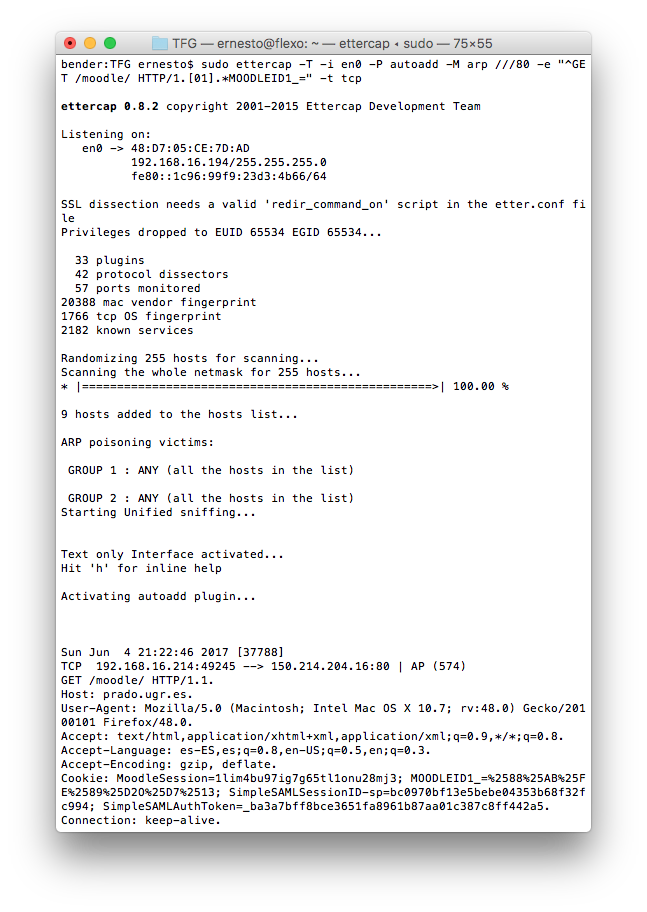
\includegraphics[width=1.0\textwidth]{../screenshots/ettercap}
\caption{Resultados del ataque mediante ettercap}
\label{fig:ettercap}
\end{figure}



\section{Análisis de disponibilidad}

Como ya hemos indicado anteriormente el 30 de enero de 2017 comenzamos a monitorizar la disponibilidad de Prado2 con la herramienta StatusCake. Como podemos ver en los periodos de disponibilidad de la figura \ref{fig:statuscake1} es una web que realmente goza de una buena disponibilidad por periodos de hasta incluso 40 días. Aunque podemos ver algunos tramos en los que la página no está accesible, estos periodos suelen ser de una duración razonable y a unas horas en las que no se espera que haya demasiados usuarios utilizando la plataforma.

\begin{figure}[h!]
\centering
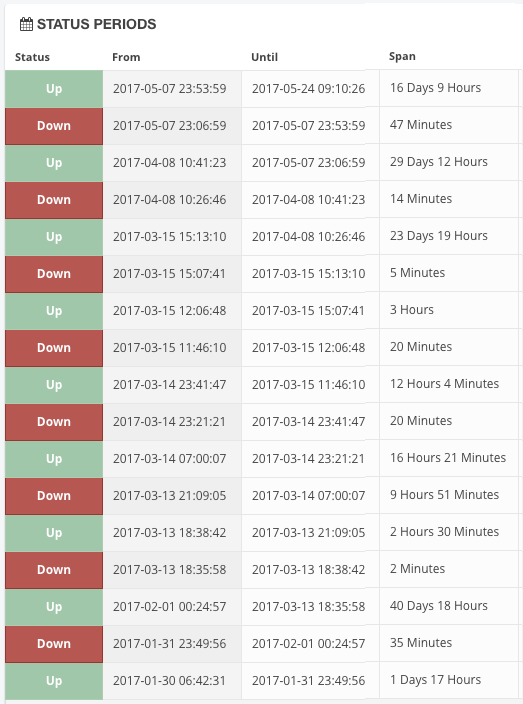
\includegraphics[width=0.8\textwidth]{../screenshots/statuscake1}
\caption{Disponibilidad medida por StatusCake}
\label{fig:statuscake1}
\end{figure}

\bigskip
Pero vemos como el 13 de marzo de 2017 hubo algún tipo de problema que se tardó bastante en solucionar y que mantuvo la plataforma sin acceso mostrando un mensaje (ver figura \ref{fig:pradocaido}) que tampoco daba a los usuarios demasiada información del problema. El mayor problema de esta caída fue el desconocimiento de los usuarios de qué estaba pasando.

\begin{figure}[h!]
\centering
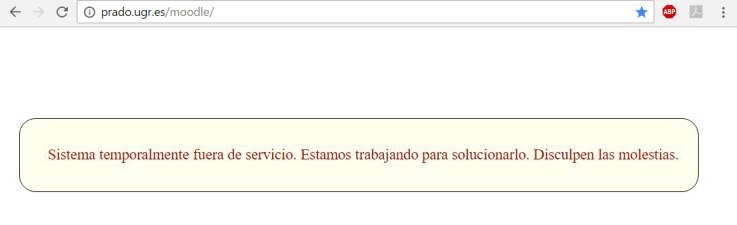
\includegraphics[width=0.8\textwidth]{../images/pradocaido}
\caption{Mensaje de error mostrado por Prado2}
\label{fig:pradocaido}
\end{figure}

\bigskip
Lo ideal en un servicio con tanto volumen de usuarios y tan crítico es informar a los usuarios de posibles cortes en el servicio. Por ejemplo, SWAD suele avisar con una notificación a todos los usuarios de futuros cortes del servicio (ver imagen \ref{fig:paroprogramadoswad}), ya que aunque el servicio se suspenda de madrugada al tener tantos usuarios siempre puede afectar a una gran parte de ellos. 

\begin{figure}[H]
\centering
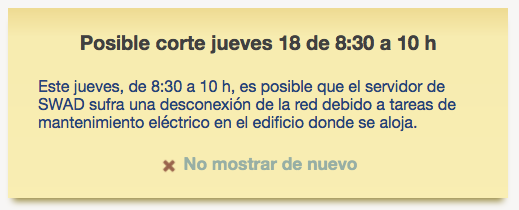
\includegraphics[width=0.8\textwidth]{../images/paroprogramadoswad}
\caption{Aviso de parada programada en SWAD}
\label{fig:paroprogramadoswad}
\end{figure}

\bigskip
En el caso de no poder prever un problema de de este tipo es recomendable al menos avisar a los usuarios por una vía alternativa como puede ser el correo institucional o las redes sociales. En el caso de la caída de Prado del día 13  de marzo aunque mucha gente alertaba en la red social Twitter de que tenían problemas para acceder a la plataforma no se recibió ninguna respuesta de la UGR hasta el restablecimiento del servicio como podemos ver en la imagen \ref{fig:tweet}. 



\begin{figure}[H]
\centering

\includegraphics[width=0.8\textwidth]{../images/tweet}
\caption{Tweet avisando del restablecimiento del servicio}
\label{fig:tweet}
\end{figure}

\bigskip
Como podemos ver en la imagen \ref{fig:statuscake2} el tiempo de respuesta del servidor es bastante bueno, ya que aunque lo ideal suelen ser 200 milisegundos en cargar la página principal Prado2 suele responder en un rango que va desde los 400 milisegundos, que está muy bien, a los 3 segundos, que se puede considerar dentro de lo aceptable. Quizá reseñar que en caso de alta demanda como puede ser el inicio del curso puede ser interesante contar con sistema de balanceo de carga para evitar los problemas que nos han comentado algunos usuarios que se han encontrado a la hora de registrarse en un grupo de prácticas, ya que al haber tanta gente conectada al mismo tiempo el sistema se ha visto colapsado. 



\begin{figure}[H]
\centering
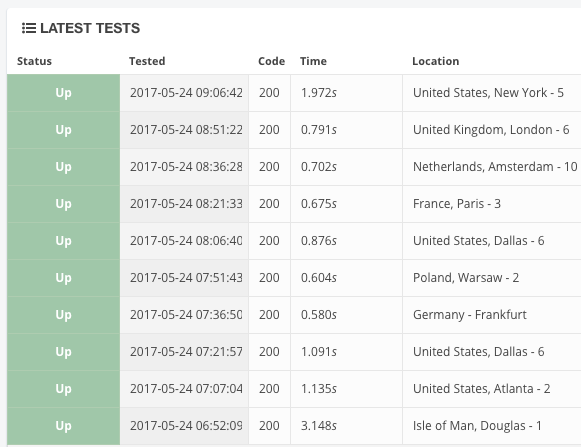
\includegraphics[width=0.8\textwidth]{../screenshots/statuscake2}
\caption{Tiempo de respuesta medido por StatusCake}
\label{fig:statuscake2}
\end{figure}


\section{Clonado de la plataforma}

Se creó el subdominio \url{http://prado.ernesto.es} en mi servidor personal y se instaló la versión 2.6.4 de moodle, luego se procedió a instalar el tema Archaius  (ver imagen \ref{fig:archaius} y a copiarle los estilos CSS en el fichero /theme/archaius/style/custom.css, copiar la imagen de cabecera (ver imagen \ref{fig:cabeceraprado} y en un tiempo mínimo teníamos funcionando un sistema casi idéntico al prado original (ver imagen \ref{fig:pradoernesto} donde agregamos unas cuantas asignaturas así como alumnos y profesores para probar las distintas opciones de moodle.

\begin{figure}[H]
\centering

\includegraphics[width=0.8\textwidth]{../screenshots/cabeceraprado}
\caption{Imagen cabecera de Prado}
\label{fig:cabeceraprado}
\end{figure}

\begin{figure}[H]
\centering
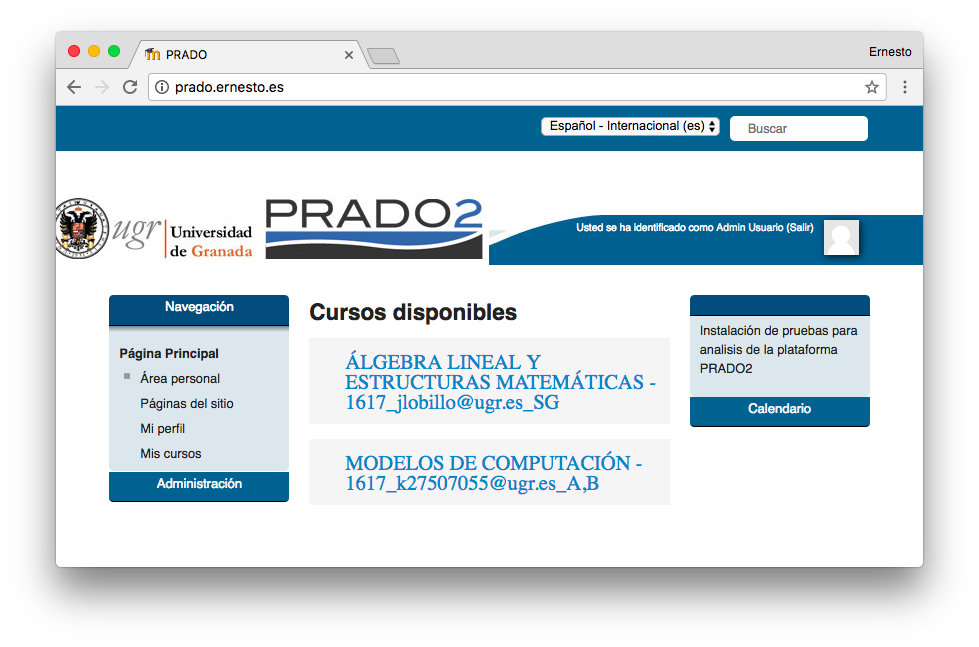
\includegraphics[width=0.8\textwidth]{../screenshots/pradoernesto}
\caption{Vista principal del clon de Prado}
\label{fig:pradoernesto}
\end{figure}

\begin{figure}[H]
\centering
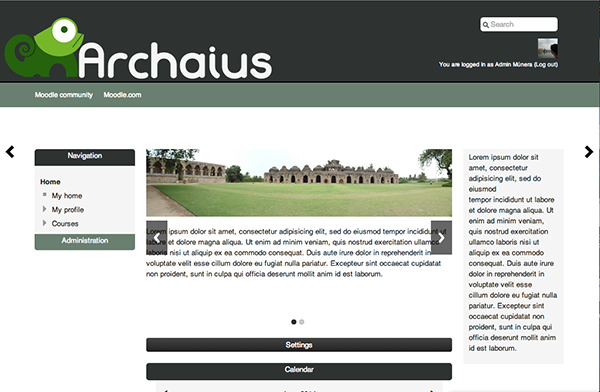
\includegraphics[width=0.8\textwidth]{../screenshots/archaius}
\caption{Captura del tema Archaius sin modificaciones}
\label{fig:archaius}
\end{figure}




\section{Realización de script GreaseMonkey}

Cuando comenzamos el proyecto pensamos en el desarrollo de una herramienta que corrigiera algunas de las carencias mas importantes de la plataforma. 

\bigskip
Como ya habíamos comprobado previamente la página no se mostraba correctamente por https porque habían rutas absolutas a elementos http y el navegador las bloqueaba por considerarlas inseguras pero si cambiábamos las urls de esos elementos la página se visualizaba correctamente.

\bigskip
Para ello escribimos un código que buscaba todas las urls que comenzaran por http y las reemplazaba por https haciendo uso de expresiones regulares. Este código funcionaba correctamente pero al hacer los cambios una vez cargada daba una sensación extraña y mucha sensación de lentitud. Aparte de esto hicimos varias pruebas y vimos que aunque la página se recargara sobre https el servidor de identificación de sesión del a ugr (\url{https://idp.ugr.es/simplesaml/module.php/core/loginuserpass.php} devolvía los valores a una página http, por lo que siempre se podían capturar los valores devueltos aunque el resto de la sesión fuera sobre un canal seguro. 

\bigskip
Además, pudimos comprobar que haciendo unos cambios mínimos en nuestro clon propio de la plataforma esta se devolvía siempre de forma correcta por https sin tener que recurrir a parches externos y siendo una mejor solución.

\bigskip
Por hacer una ultima prueba quisimos probar si sería posible hacer cambios estéticos en la plataforma por lo que inyectamos el código \texttt{\$( '.block' ).css( 'display' , 'block' );} que simplemente le dice mediante javascript que despliegue todos los bloques laterales de la página lo cual hacía que la navegación fuese un poco menos caótica pero al igual que lo anterior sin llegar a ser una solución del todo viable y limitándose a un simple parche temporal así que finalmente descartamos el desarrollo del script, de todas formas hemos considerado incluir lo desarrollado en los anexos.


\section{Herramienta hardware para robo de sesiones}

Para desarrollar la herramienta utilizamos un viejo router Huawei HG556a de Vodafone al que le instalamos el firmware libre OpenWRT \cite{openwrt}. 

\bigskip
Una vez instalado el firmware configuramos dos interfaces inalámbricas virtuales. La primera interfaz se configuró en modo cliente que conectamos a la red \textit{eduroam} haciendo uso de los certificados pertinentes y mi cuenta personal de usuario de la UGR. La segunda interfaz se configuró en modo punto de acceso, creando una red wifi sin contraseña de nombre \textit{eduroam\_pruebas} y agregamos las reglas necesarias a iptables para que redirigiera el trafico de una interfaz a otra por lo que los clientes que se conectaban a la red wifi \textit{eduroam\_pruebas} realmente estaban saliendo a internet por la red \textit{eduroam} pero con la salvedad de que podíamos espiar el tráfico que pasaba por la red. A este tipo de dispositivos de les denomina \textit{honeypot} (tarro de miel). 

\bigskip
Instalamos el programa \textit{ettercap} que utilizamos durante la auditoría de seguridad y lo configuramos para empezar a capturar información. A los pocos minutos de empezar a capturar nos dimos cuenta que el limitado espacio del dispositivo iba a ser un problema, pues el HG556a cuenta con sólo 16MB de ROM y 64MB de RAM a todas luces insuficiente para una captura de este tipo así que conectamos una unidad USB de 16GB, la montamos como lectura/escritura y solucionamos el problema del espacio. 

\bigskip
Una vez vimos que el sistema funcionaba probando a secuestrar nuestras sesiones fuimos a la sala de libre acceso que hay al lado de la biblioteca de la ETSIIT en la que habían unos 15 estudiantes, conectamos el aparato, lo disimulamos entre unas mochilas y volvimos a comprobar que todo funcionaba correctamente y podíamos capturar nuestras variables de sesión si nos conectábamos a prado a través de esta red. 

\bigskip
Hicimos un poco de ingeniería social comentando en voz alta que estaban probando una nueva red wifi que se llamaba \textit{eduroam\_pruebas} que iba mucho más rápida y nos pusimos a esperar. En dos horas que estuvimos en la sala contabilizamos un total de 37 clientes conectados al router, de los cuales 18 se conectaron a prado y de todos ellos pudimos capturar sus variables de sesión. 

\bigskip
Evidentemente aunque vimos los valores de las variables de sesión en ningún momento hicimos uso de ellas para suplantar la identidad de nadie, ya que no contábamos con la autorización debida, todo fue un ejercicio confirmar nuestras sospechas de que era realmente fácil realizar un ataque a la plataforma.




